\section{Steering as a Variation Operator}\label{sec:steering}
\pages{2.5}

\plan{Steering vector $c\cdot a\cdot d$ added to the residual stream at
every generated token: unit direction $d$, dose $c$, scale $a$ (typical
feature activation or residual norm). Controls: random unit directions
at the same norm, and a resample with a new seed. Directions: SAE
decoder columns, and contrastive mean differences on a labelled corpus
of 4,712 algorithms (concept present vs.\ absent; most vs.\ least
exploratory), the exploration direction residualised on the concept
labels.}

\subsection{Concept levers}
\begin{itemize}
  \item Of the SAE features, only swarm and gradient steer their concept
    cleanly (at $0.5\times$); most do nothing or break the code.
  \item Of ten contrastive rare-concept directions, four insert their
    concept (covariance, local search, simulated annealing, surrogate:
    +0.31 to +0.44), at a failure cost; a direction that \emph{reads} a
    concept well is often not one that \emph{writes} it.
  \item In \llamea (4 arms $\times$ 8 seeds $\times$ 100): the swarm
    lever puts a PSO in 99\% of its children (control 15\%), as novel as
    the \emph{new} prompt with fewer failures, but these children are
    selected away; run-level diversity and best \aocc unchanged.
\end{itemize}
\src{exp05\_steering: screen, contrast-c, llamea}

\subsection{An exploration dial}
\begin{itemize}
  \item Residualised exploration direction at layer 27: the children's
    measured exploration rises by 20 points per unit dose (95\% CI 6 to
    36) and intensification falls, replicated on new prompts (1,152
    children); a random direction at the same norm does not move it
    ($-3$, CI $-15$ to 7; Fig.~\ref{fig:dial}).
  \item Fine but small: $\pm0.4$ spans about 19 points; a prompt
    instruction spans 59.
\end{itemize}
\src{exp05\_steering: contrast-b, dial}

\begin{figure}[t]
  \centering
  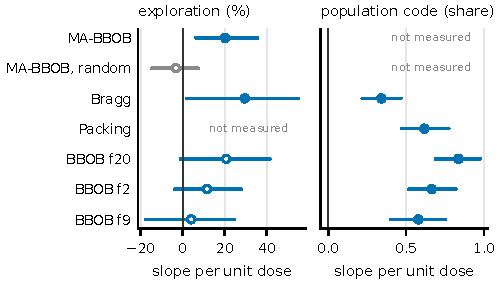
\includegraphics[width=\columnwidth]{figures/dial}
  \caption{The exploration dial in single-generation screens: slope per
    unit dose of the measured exploration of the generated code (left)
    and of the share of population-based code (right), initial and
    refine prompts pooled, with 95\% bootstrap intervals; filled marks
    exclude 0. The direction is derived from MA-BBOB code only.
    Packing calls no black box, so its exploration is not measured.}
  \Description{Two forest plots. Left: the exploration slope is about
    +20 on MA-BBOB and +30 on Bragg (both significant), +21, +12 and +4
    on BBOB f20, f2 and f9 (not significant), and about 0 for a random
    direction. Right: the population-code share rises by 0.35 to 0.84
    per unit dose on all five transfer problems.}
  \label{fig:dial}
\end{figure}

\subsection{Transfer to new problems}
\plan{The dial derived from MA-BBOB code, applied unchanged to \llamea
prompts for mini-Bragg photonics (10 layers), unit-square circle packing
($n=26$) and three BBOB functions in 20-D (Sec.~\ref{sec:setup}); 32
initial and 32 refine samples per dose ($\pm0.2$, $\pm0.4$, none,
random direction).}
\begin{itemize}
  \item The design-space effect transfers everywhere: per unit dose the
    share of population-based code rises by 0.35 (Bragg) to 0.84 (f20),
    DE rises and local search or gradient code falls
    (Fig.~\ref{fig:dial}, right).
  \item The behaviour effect is weaker: measured exploration +30 per unit
    dose on Bragg (CI 2 to 55), +21 on f20 ($-1$ to 42), +12 on f2 and
    +4 on f9 (n.s.).
  \item Code quality in one generation: higher \aocc with the dose on
    f2 (+0.083, CI 0.043 to 0.126) and f9 (+0.058, 0.014 to 0.102),
    flat on f20, Bragg (+0.04 at +0.4, n.s., 64 samples) and packing;
    on packing the explore side cuts failures ($-0.37$ per unit dose).
  \item A probe of exploration trained on MA-BBOB code does not transfer
    (Spearman $-0.08$ with measured exploration on Bragg): the dial
    transfers, its readout does not.
\end{itemize}
\src{exp05\_steering: transfer-\{bragg,packing,bbob-f20,bbob-f2,bbob-f9\}}

\subsection{The dial in the closed loop}
\plan{\llamea arms (Sec.~\ref{sec:setup}): control; the dial at fixed
dose $+0.3$ (explore) or $-0.3$ (exploit); anneal ($+0.3\to-0.3$ over
the budget); a random direction; an \emph{adaptive dial}, unsteered
initial population and then a stagnation rule (dose $-0.1$ after a child
that improves the best, $+0.025$ otherwise, clipped to $\pm0.3$); and
the obvious alternative, a \emph{prompt} sentence asking for strong
exploration or exploitation (the sentence that elicited the corpus).
Differences are paired by seed, 95\% bootstrap CIs.}

\paragraph{MA-BBOB (Table~\ref{tab:mabbob}, Fig.~\ref{fig:budget200}).}
\begin{itemize}
  \item Exploit is reliably harmful: best \aocc $-0.24$ (CI $-0.35$ to
    $-0.12$) at 100 evaluations and $-0.19$ ($-0.30$ to $-0.07$) at 200;
    explore $-$ exploit $+0.24$ ($+0.16$ to $+0.32$, 14/16 seeds) at 200;
    exploit writes 18 algorithm families per run, control 26.
  \item The adaptive dial is the best arm and the only one that widens
    the search (+6.4 families, CI 1.6 to 10.9; more failures, +0.06).
    Its gain over control is +0.06 ($-0.01$ to $+0.14$) at 100 and
    becomes significant at 200: +0.08 (+0.02 to +0.14, 12/16 seeds).
    The success rate stays far below the rule's target, so in practice
    it is ``explore after an unsteered start'' (mean dose +0.25).
  \item Every arm still improves from 100 to 200 evaluations (+0.04 to
    +0.09, all CIs above 0): the steering gap is not a faster start.
  \item The fixed explore dial, anneal, the random direction and both
    prompts are not distinguishable from control ($|\Delta|\le0.05$ at
    200). The prompts move the measured exploration more than the dial
    (+19 vs.\ +8 points) but cut 7--12 families and leave a lexical
    imprint (83\% step-size adaptation under the exploit prompt vs.\ 21\%).
\end{itemize}
\src{exp05\_steering: llamea-dial, llamea-stage1(-seeds), budget200}

\begin{table}[t]
  \caption{Steered \llamea on MA-BBOB: best \aocc at 100 and 200
    evaluations, families of algorithms written (budget 100), mean over
    16 seeds; $\Delta$ is the paired difference to control at 200 with
    its 95\% bootstrap CI. Bold: CI excludes 0.}
  \label{tab:mabbob}
  \small
  \setlength{\tabcolsep}{4pt}
  \begin{tabular}{lrrrr}
    \toprule
    Arm & @100 & @200 & $\Delta$@200 [95\% CI] & families\\
    \midrule
    control & 0.64 & 0.68 & -- & 26.4\\
    adaptive dial & 0.70 & 0.75 & \textbf{+0.08} [+0.02, +0.14] & 32.9\\
    dial explore & 0.66 & 0.73 & +0.05 [$-$0.04, +0.13] & 28.1\\
    dial exploit & 0.40 & 0.49 & \textbf{$-$0.19} [$-$0.30, $-$0.07] & 17.9\\
    dial anneal$^*$ & 0.62 & 0.70 & +0.02 [$-$0.07, +0.11] & --\\
    random dir.$^*$ & 0.58 & 0.66 & $-$0.02 [$-$0.11, +0.07] & --\\
    prompt explore & 0.62 & 0.69 & +0.01 [$-$0.07, +0.08] & 14.2\\
    prompt exploit & 0.59 & 0.63 & $-$0.05 [$-$0.12, +0.03] & 19.3\\
    \bottomrule
  \end{tabular}\\[2pt]
  \raggedright\footnotesize $^*$anneal is run at budget 200, so its @100
  is mid-schedule; 8 of the 16 random-direction runs too.
  \todo{families for anneal/random on 16 seeds}
\end{table}

\begin{figure}[t]
  \centering
  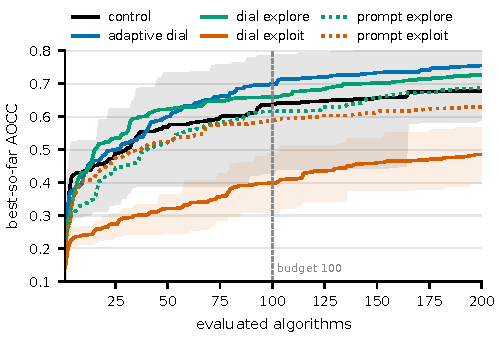
\includegraphics[width=\columnwidth]{figures/budget200}
  \caption{Best-so-far \aocc of steered \llamea on MA-BBOB, mean over 16
    seeds (bands: interquartile range of control and the exploit dial).
    Runs to the left of the dashed line are the budget-100 campaigns;
    all were continued to 200 evaluations.}
  \Description{Line chart over 200 evaluations. The adaptive dial ends
    highest at 0.75, the explore dial at 0.73, control at 0.68, the
    prompts at 0.63 to 0.69, and the exploit dial far below at 0.49.}
  \label{fig:budget200}
\end{figure}

\paragraph{Bragg and packing (6 seeds).}
\begin{itemize}
  \item Nothing beats the unsteered control. Steering the initial
    population breaks it (Bragg: 96--100\% of steered initial
    algorithms fail vs.\ 71\%), and Bragg runs are bimodal (control
    finds the quarter-wave stack in 4/6 runs, exploit and explore in
    1/6). The adaptive dial, which leaves the initial population alone,
    does not rescue Bragg ($-0.29$, CI $-0.50$ to $-0.05$).
  \item On packing every push of the behaviour costs constraint
    handling, steering or prompt alike: strictly feasible packings fall
    from 0.37 to about 0.1 (dial) and by 0.16--0.23 (prompts). Anneal is
    the only neutral arm.
\end{itemize}
\src{exp05\_steering: llamea-dial-\{bragg,packing\},
llamea-stage1-\{bragg,packing\}}

\paragraph{BBOB 20-D: a pre-registered landscape test
(Table~\ref{tab:bbob}).}
\plan{Prediction registered before the runs: on the multimodal f20,
explore $>$ control $>$ exploit; on the unimodal f2 and f9, exploit
$\ge$ control $>$ explore. 6 arms $\times$ 10 seeds $\times$ 100;
final best validated on 16 held-out instances.}
\begin{itemize}
  \item The prediction fails on all three functions. f20: all arms end
    at 0.24--0.26; explore has the best anytime curve (area +0.025, CI
    +0.004 to +0.057). f2: control $\approx$ adaptive $\ge$ explore $>$
    exploit (control $-$ exploit +0.21, CI $-0.00$ to $+0.40$). f9:
    explore is best (+0.013, CI +0.007 to +0.020, 10/10 seeds).
  \item The dial acts on the design space, not on the optimiser's
    behaviour: exploit cuts the families written by 9--13 (all
    significant) and nearly removes DE and crossover. On f2 runs are
    bimodal, and 87\% of the breakthrough runs' best algorithms use DE
    (stuck runs: 16\%); exploit-steered runs rarely find them (2/10 vs.\
    6/10).
  \item Exploit lowers the measured exploration on f20 ($-21$ points)
    but not the best; the explore side never hurts.
  \item The final algorithms generalise: train $-$ test gap $\le0.021$
    \aocc, no failures on the held-out instances.
\end{itemize}
\src{exp05\_steering: llamea-bbob-\{f20,f2,f9\}}

\begin{table}[t]
  \caption{BBOB 20-D, best \aocc of the run (training instances 10--14)
    and of its best algorithm on held-out instances 15--30, mean over
    10 seeds. Pre-registered prediction: f20 explore best; f2 and f9
    exploit best. Bold: best arm.}
  \label{tab:bbob}
  \small
  \setlength{\tabcolsep}{3.5pt}
  \begin{tabular}{lrrrrrr}
    \toprule
    & \multicolumn{2}{c}{f20 (multimodal)} & \multicolumn{2}{c}{f2
    (ellipsoid)} & \multicolumn{2}{c}{f9 (Rosenbrock)}\\
    \cmidrule(lr){2-3}\cmidrule(lr){4-5}\cmidrule(lr){6-7}
    Arm & train & test & train & test & train & test\\
    \midrule
    control & 0.240 & 0.236 & 0.593 & \textbf{0.578} & 0.333 & 0.328\\
    adaptive dial & \textbf{0.259} & \textbf{0.257} & \textbf{0.598} &
      0.577 & 0.331 & 0.327\\
    dial explore & 0.258 & 0.252 & 0.537 & 0.541 & \textbf{0.347} &
      \textbf{0.336}\\
    dial exploit & 0.255 & 0.247 & 0.381 & 0.381 & 0.337 & 0.331\\
    prompt explore & 0.254 & 0.251 & 0.352 & 0.344 & 0.333 & 0.327\\
    prompt exploit & \textbf{0.259} & 0.252 & 0.359 & 0.356 & 0.340 & 0.333\\
    \bottomrule
  \end{tabular}
\end{table}
